\documentclass{article}
\usepackage[utf8]{inputenc}
\usepackage[T1]{fontenc}
\usepackage{graphicx}
\usepackage{amsmath}
\usepackage{wrapfig}
\usepackage[top=1in, bottom=1.25in, left=1.1in, right=1.1in]{geometry}

\title{Reporte - Actividad 5: Preparando Datos con Ayuda de Emacs}
\author{García Monge Itzel Alexia}
\date{06 de Marzo, 2018}

\begin{document}
\maketitle
\section{Introducción}
En el siguiente reporte se encuentra el procedimiento realizado para limpiar y graficar la relación entre los datos CAPE y precipitación de la estación Abha ubicada en el Medio Oriente. Para esto, se buscaron y utilizaron comandos de Emacs, así como la utilización nuevamente de Pandas en Jupyter Notebook para darles el formato necesario. Además, se utilizó una nueva Biblioteca para graficar de formas más diversas en Jupyter con Matplotlib.

\section{Conceptos Físicos}
\subsection{Convective Available Potential Energy (CAPE)}
La  cantidad de energía disponible para la convección, o CAPE por sus siglas en inglés, es energía por unidad de masa y no posee las medidas típicas de otros índices de inestabilidad, optando por la unidad de Jules/Kilogramos. La energía puede manifestarse de diversas formas con la habilidad de transformarse de un tipo a otro, ya sea de forma potencial, cinética, electrostática, y hasta elástica. 
 
La convección es un proceso por el cual la atmósfera, o un fluido en general, trata de redistribuir los desequilibrios que se producen en su seno por el calor, temperatura y humedad mediante corrientes verticales relativamente intensas, tanto ascendentes como descendentes. Por esta razón, CAPE está directa y teóricamente relacionada con la velocidad vertical potencial máxima dentro de una corriente ascendente o descendente. Los valores más altos indican un mayor potencial para tiempo severo.

\subsection{Precipitación (PW)}
El agua precipitable es la cantidad de agua, expresada como altura o masa, que se obtendría si todo el vapor de agua contenido en una columna específica de la atmósfera, de sección transversal horizontal unitaria, se condensase y precipitase.

\section{Proceso de Limpieza}
Se toma el documento $df2017.csv$ de la actividad anterior y se usa un \textbf{grep} para que solo se obtenga la información de la precipiración y la CAPE de la tabla de datos, redireccionando los datos para que no se impriman en pantalla de la terminal, moviéndolos a un nuevo archivo llamado $df2017 PW.cvs$. Este nuevo archivo es el que se va a manejar por el resto de la actividad.

Lo que queremos del archivo son la fecha y los valores de la CAPE y la precipitación a las 00Z y 12Z horas de todo el año. Si abrimos el documento en $Emacs$, observamos que aunque se hayan filtrado esos valores del archivo anterior, aún queda mucha basura que no se necesita. Un ejemplo sería el título de la estación o la indicación de que se dará el valor de CAPE o precipitación. Hay que tener cuidado de no borrar las horas de la medición, ya que aunque no aparezcan en el formato de la tabla final son muy importantes para la limpieza de datos.

Para eliminar los renglones que se repiten una cantidad enorme de veces durante todo el documento y no son necesarios se usan los comandos de $Emacs$. Usamos \textbf{ctrl + space bar} para seleccionar el área que queremos eliminar, observando que por donde se pasa se marca con azúl. Ya que seleccionamos todo lo que no queremos conservar en el archivo usamos el comando \textbf{ctrl + w} para que borre ($wipe$) lo seleccionado, pero lo traemos de vuelta con \textbf{ctrl + y} para que se vacíe la memoria y quedé guardado en el $junk$. Regresamos al inicio del documento con \textbf{esc + <} para llamar a query replace \textbf{esc + \%}.

Cuando llamaos a query replace, aparece en la parte inferior de $Emcas$ una pequeña barra, la seleccionamos y vaciamos la memoria del $junk$ que pusimos con \textbf{ctrl + y} una vez. Se puede apreciar como todo lo que se había seleccionado y borrado en el documento aparece en la barra. Aplastamos \textbf{enter} y escribimos lo que sea que queramos reemplazar en lugar de esa línea, si deseamos simplemente borrarlo solamente volvemos a presionar \textbf{enter}. 

Con eso, todas las veces que esa línea aparece en el documento serán seleccionadas en $Emacs$, para reemplazar todas ellas por el valor que volviste a meter se escribe \textbf{!} en la barra. Automáticamente todos los valores serán cambiados y la barra incluso indicará cuántas veces se cambió el valor.

Repetimos un proceso similar para cambiar el nombre de los meses $Jan, Feb,...,Dec$ y añadir comas entre los datos. La única diferencia es que se debe de tener cuidado de no presionar \textbf{enter} nuevamente después de vaciar lo que queremos borrar en la barra inferior, en cambio, se escribe el número del mes o una coma, respectivamente.

Al finalizar el proceso, tendremos una tabla algo similar al resultado final que queremos obtener, pero no está completamente terminada. Se nos pide organizar en un solo documento los datos que ocurrieron a las 12Z horas y en otro documento los datos que ocurrieron a las 00Z. Para eso se abre un terminal en la carpeta de la $Actividad 5$ y se usa el \textbf{grep} para filtrar todos los valores que solamente sean de esas horas, redireccionando su impresión a un documento específico. Al final contaremos con dos documentos nuevos: $df2017 PW 00Z.csv$ y $df2017 PW 12Z.csv$.

Una vez creados ambos documentos, se puede tomar como terminada satisfactoriamente la limpia de datos en $Emacs$ y proseguir a dar formato con $Pandas$ recurriendo a la herramienta de $Jupyter Notebook$, la cual ya ha sido utilizada y analizada en actividades pasadas.

\section{Análisis de Datos}
Al tener los datos separados por archivos y de la manera deseada, se abre una terminal en la carpeta $Actividad5$ y se abre el Kernel de $Jupyter Notebook$. Abrimos un archivo de Python nuevo e importamos las bibliotecas de $Pandas$, $Numpy$ y $Datetime$.

Como siempre que se quiere manejar un archivo ya existente, leemos los documentos usando $pandas$. Denominamos al archivo con las horas de 12Z $df12$ y al archivo con las horas 00Z $df00$. 

Con pandas, ya podemos darle el último toque a nuestras tablas, es decir, podemos darles un encabezado y un formato. Además, convertimos la columna $CAPE$ que aparece como objeto a número para poder leer sus datos al momento de graficar y cambiamos los datos de las fechas a una variable temporal denominada $NDate$ en donde se ordenara la fecha por año-mes-día.

    \begin{center}
    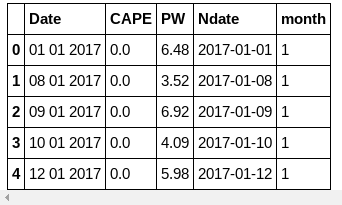
\includegraphics[height=4.5cm]{datos00.png}
    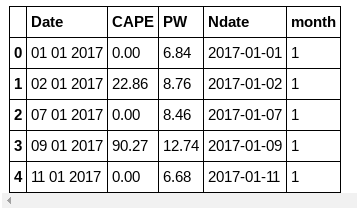
\includegraphics[height=4.5cm]{datos12.png}
    \end{center}
    
Ahora los archivos por fin están completamente listos para graficarse. Estas deben ser una por cada hora, es decir, se grafica para $df12$ y otra para $00Z$ en todos los casos. La primera gráfica que queremos hacer es una gráfica de caja, por lo que necesitamos importar dos bibliotecas a Pyhton: $matplotlib$ y $Seaborn$. 

Una vez importadas podemos crear gráficas de cajas de la CAPE:

\begin{verbatim}
ax = sns.boxplot(x="month", y="CAPE", data=df12)
plt.show()
\end{verbatim}

Y de la precipitación:

\begin{verbatim}
plt.show()
ax = sns.boxplot(x="month", y="PW", data=df12)
\end{verbatim}

Las gráficas de cajas graficaron una cosa en específico, ya sea una gráfica con la CAPE o una con la precipitación, pero el punto de la actividad es ver si tiene alguna relación. Entonces necesitamos una gráfica de correlación en donde podamos graficar una respecto a la otra, para eso seguimos usando $Seaborn$. 

\begin{verbatim}
sns.set(style="darkgrid", color_codes=True)

g = sns.jointplot("CAPE", "PW", data=df12, kind="reg",
                   color="r", size=7)
plt.show(g)
\end{verbatim}

La última gráfica que se desea construir es una regresión lineal de todo el año.

\begin{verbatim}
g = sns.lmplot(x="CAPE", y="PW", hue="month",
               truncate=True, size=5, data=df00)
plt.show(g)
\end{verbatim}

\section{Resultados}
Para la gráfica de cajas se obtuvieron cuatro gráficas. En estas gráficas se puede apreciar una recta vertical, este el el rango total de los datos en cada mes, dentro de ellos aparece una "caja", las esquinas de la caja representan el primer y tercer cuartil--los cuartiles siendo la mediana del primer segmento antes de la mediana--mientras que la línea dentro de esa caja representa el segundo cuartil, mejor conocido como la media. Los puntos obervados fuera o entre medio del rango se llaman datos atípicos. Dentro de la caja se encuentran el 50\% de los datos, un 25\% se enceuntra en la parte superior del rango que queda y el último 25\% se encuentra en la parte inferior.

Las primeras dos fueron realizadas graficando CAPE, empezando con 00Z y siguiendo con 12Z:

	\begin{center}
    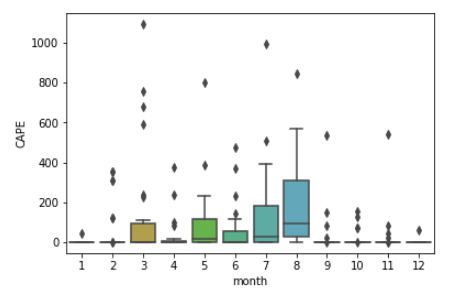
\includegraphics[height=5cm]{cajaCape00.png}{00Z}
    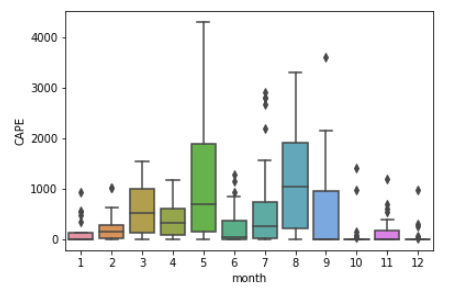
\includegraphics[height=5cm]{cajaCape12.png}{12Z}
    \end{center}

Se puede observar a primera vista que en ambas gráficas que los valores están sesgados. Esto significa que los datos se inclinan más a unos valores en específico. Los datos puedes estar sesgados si la media no se encuentra centrada en la caja o si la caja misma no se encuentra centrada en el rango.

En la gráfica de 00Z no se cuentan con suficientes datos en la mayoría de los meses, habiendo más sondeos realizados durante los meses de mayo, julio y agosto. Es en estos meses que se puede observar bien los tres cuartiles, habiendo un sesgo grande hacia abajo. En general, hubo una gran cantidad de datos atípicos durante todo el año.

En la gráfica de 12Z son mínimos los meses que no forman cajas, y los datos atípicos tiene mucha precisión entre sí. Aún así, se cuenta con un gran sesgo hacia abajo con el la gráfica de 00Z, mayo siendo el ejemplo más claro de esto.

En las siguientes gráficas de caja se graficó la precipitación (PW), siguiendo el mismo orden de 00Z y 12Z tenemos las gráficas:

	\begin{center}
    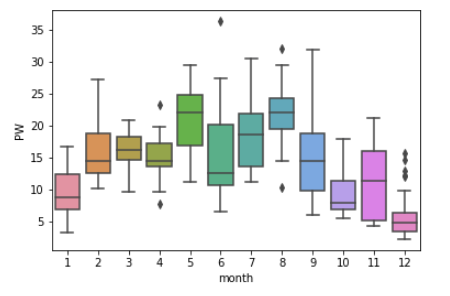
\includegraphics[height=5cm]{cajaPW00.png}{00Z}
    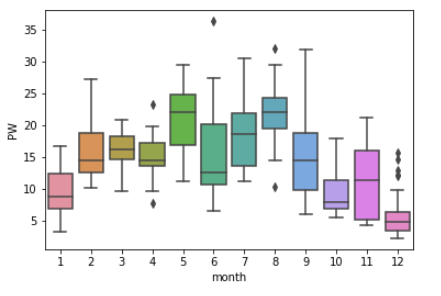
\includegraphics[height=5cm]{cajaPW12.png}{12Z}
    \end{center}

El rango en las gráficas de precipitación se encuentran mucho más centradas que las gráficas de CAPE. Aún sigue habiendo datos atípicos, pero estos son mínimos a comparación de las gráficas anteriores, en especial con la de 00Z.

La gráfica de 00Z muestra datos centrados o con un sesgo hacia abajo, pero no un sesgo tan notorio como en las gráficas anteriores, siendo este más ligero. Todos los meses cuentan con una caja y media bien definidas y solamente cuatro meses cuentan con datos atípicos en ellos.

La gráfica de 12Z también se centra más aunque sigue teniendo un sesgo algo notable hacia abajo. Como su gráfica hermana, cuenta con solamente cuatro meses presentando datos atípicos, cajas y medias bien definidas, y una cantidad de datos considerables.

Además de presentar gráficas de cajas, se realizaron dos gráficas de relación entre la CAPE y precipitación entre los datos de 00Z y 12Z, respectivamente. Obteniendo las gráficas:

	\begin{center}
    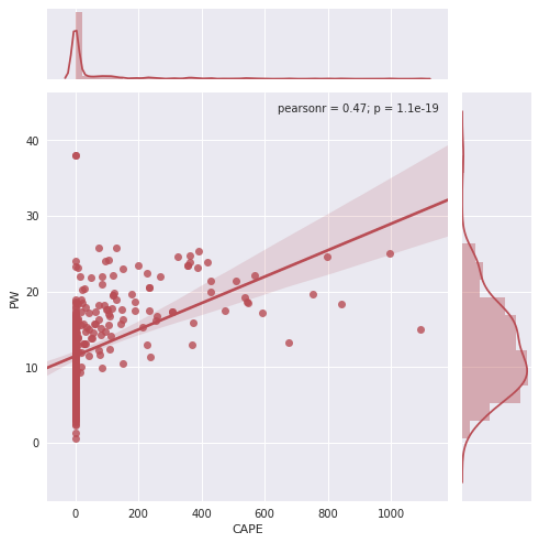
\includegraphics[height=10cm]{relacion00.png}{00Z}
    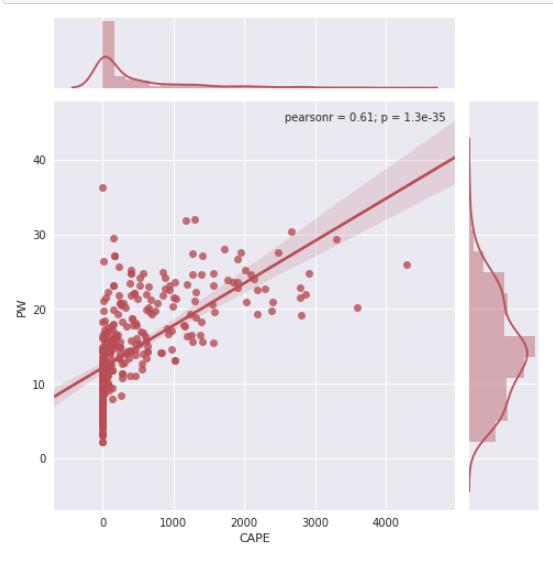
\includegraphics[height=10cm]{relacion12.png}{12Z}
    \end{center}
    
La gráfica muestra si está relacionada CAPE con el agua precipitada, creando una recta que mejor se ajuste a todos los datos con la menor distancia entre los datos y la gráfica posible. La relación en la gráfica de 00Z es de  r=0.41, lo cual se puede interpretar el coeficiente de correlación lineal, es decir, que tan linealmente relacionada está relacionada CAPE con la precipitación. Mientras que en la gráfica de 12Z se tiene una relación de r=0.61 Esto quiere decir que cuando CAPE crece, también lo hace la precipitación con una relación de 0.41 y 0.61.

Por último, se deseo realizar gráficas de un modelo de regresión lineal en todo el año. El objetivo era observar si se podía tener el agua precipitable como una función lineal del CAPE. Las gráficas obtenidas fueron:

	\begin{center}
    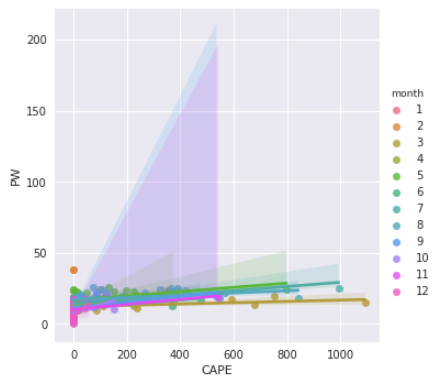
\includegraphics[height=9cm]{regresion00.png}{00Z}
    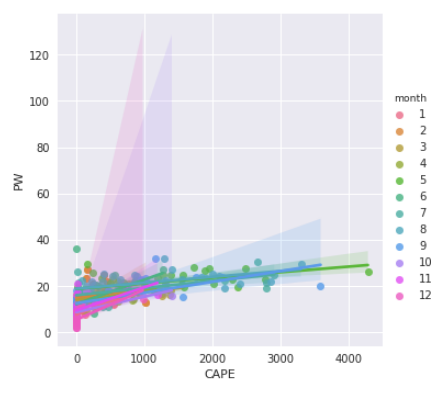
\includegraphics[height=9cm]{regresion12.png}{12Z}
    \end{center}

En estas gráficas se crea una recta para cada mes, teniendo un total de doce rectas, además se pueden apreciar triángulos que siguen a cada recta, estos son la distribución de los datos, lo que quiere que decir que se muestra qué tan acumulados se encuentran los datos en ese mes. En la gráfica de 00Z se tiene una mayor acumulación en el mes de julio, mientras que diciembre es el más con más acumulación en la gráfica de 12Z. En conclusión, al obtener una gráfica sabemos que es posible hacer que el agua precipitable se pueda escribir cono una función lineal de CAPE, pero genera gráficas que no tienen mucho sentido.

\section{Conclusiones}
La limpieza y graficación de datos no es un trabajo que puede realizarse en un solo programa. Hay veces que resulta más eficiente utilizar varias herramientas de programación que se especializan cada una en algo para conseguir lo que uno desea que tratar de recrear todo en un solo lugar. En esta actividad se recurrió al uso de los comandos de $Emacs$--de los cuales quedaron demasiados sin usar--observando que su uso es muy práctico al crear tablas y limpiar datos de una manera muy rápida y sin muchas complicaciones. Se utilizó bash en la terminal para filtrar los datos que se querían limpiar así como crear dos documentos nuevos con las horas específicas utilizando un solo comando. Además, se utilizó Python para dar un formato a ls tablas, además de crear gráficas complejas de manera rápida, colorida y muy bien hechas.

\section{Bibliografía}
\begin{itemize}
\item Curso sobre interpretación de mapas meteorológicos: la CAPE (Convective Available Potencial Energy). (2013, May 27). Retrieved March 03, 2018

$https://www.tiempo.com/ram/800/curso-sobre-interpretacin-de-mapas-meteorolgicos-el-cape-convective-available-potencial-energy/$

\item Convective Available Potential Energy (CAPE) (Meteorología e hidrología (inglés-español)). Retrieved March 03, 2018

$https://glosarios.servidor-alicante.com/meteorologia-hidrologia_en-es/convective-available-potential-energy-cape$

\item A. Agua precipitable. Retrieved March 03, 2018

$http://www.aguamarket.com/diccionario/terminos.asp?$

\end{itemize}

\section{Apéndice}
\begin{enumerate}
\item ¿Cómo se te hizo esta actividad? ¿Compleja, Difícil, Sencilla?
Al principio, ya que no entendía del todo los comandos de $Emacs$, me confundí fácilmente con la limpieza del documento. Al final, al entender con un pequeño ejemplo de por medio, la función de los comandos, pude realizar la actividad de manera fácil.

\item¿Qué te llamó más la atención?
La forma rápida en la que se puede limpiar un documento en $Emacs$, en especial el como dejamos en forma de tabla al documento al final con el simple hecho de eliminar lo que no queríamos. Me pareció muy poderoso y algo que nos puede servir mucho en el futuro.

\item¿Qué parte fue la que menos te interesó hacer?
No me llamo la atención repetir tantas veces el proceso de limpieza una vez que me di cuenta que faltaban comas entre dos columnas, me gustaría saber de una forma más interesante de arreglar ese problema sin demorar tanto tiempo.

\item¿Cómo mejorarías esta actividad? ¿Qué le faltó? ¿Qué sobró?
Me gustaría que la próxima vez que se realice la actividad se pueda explicar un poco más lo que son y lo que hacen las gráficas que se generaron en $Jupyter Notebook$, ya que aunque eran fáciles de recrear no se tenía mucho contexto de ellas. 

\item¿Hasta este punto, que te parece el uso de Jupyter para programar en Python? 
Me parece una herramienta muy cómoda para graficar y terminar de darle los últimos toques a la limpieza de datos. Definitivamente fue más difícil limpiar los datos desde cero usando $Python$ solamente, pero al usarlo en este actividad con el que da los toques finales a la table es mucho más cómodo. Sin mencionar que me parece muy interesante descubrir que existen muchas bibliotecas que aún no hemos visto las cuales pueden generar gráficas más complejas de manera tan rápida.

\end{enumerate}

\end{document}
